\documentclass{beamer}
\mode<presentation>
\usepackage{amsmath,amssymb,mathtools}
\usepackage{textcomp}
\usepackage{gensymb}
\usepackage{adjustbox}
\usepackage{subcaption}
\usepackage{enumitem}
\usepackage{multicol}
\usepackage{listings}
\usepackage{url}
\usepackage{graphicx} % <-- needed for images
\def\UrlBreaks{\do\/\do-}

\usetheme{Boadilla}
\usecolortheme{lily}
\setbeamertemplate{footline}{
  \leavevmode%
  \hbox{%
  \begin{beamercolorbox}[wd=\paperwidth,ht=2ex,dp=1ex,right]{author in head/foot}%
    \insertframenumber{} / \inserttotalframenumber\hspace*{2ex}
  \end{beamercolorbox}}%
  \vskip0pt%
}
\setbeamertemplate{navigation symbols}{}

\lstset{
  frame=single,
  breaklines=true,
  columns=fullflexible,
  basicstyle=\ttfamily\tiny   % tiny font so code fits
}

\numberwithin{equation}{section}

% ---- your macros ----
\providecommand{\nCr}[2]{\,^{#1}C_{#2}}
\providecommand{\nPr}[2]{\,^{#1}P_{#2}}
\providecommand{\mbf}{\mathbf}
\providecommand{\pr}[1]{\ensuremath{\Pr\left(#1\right)}}
\providecommand{\qfunc}[1]{\ensuremath{Q\left(#1\right)}}
\providecommand{\sbrak}[1]{\ensuremath{{}\left[#1\right]}}
\providecommand{\lsbrak}[1]{\ensuremath{{}\left[#1\right.}}
\providecommand{\rsbrak}[1]{\ensuremath{\left.#1\right]}}
\providecommand{\brak}[1]{\ensuremath{\left(#1\right)}}
\providecommand{\lbrak}[1]{\ensuremath{\left(#1\right.}}
\providecommand{\rbrak}[1]{\ensuremath{\left.#1\right)}}
\providecommand{\cbrak}[1]{\ensuremath{\left\{#1\right\}}}
\providecommand{\lcbrak}[1]{\ensuremath{\left\{#1\right.}}
\providecommand{\rcbrak}[1]{\ensuremath{\left.#1\right\}}}
\theoremstyle{remark}
\newtheorem{rem}{Remark}
\newcommand{\sgn}{\mathop{\mathrm{sgn}}}
\providecommand{\abs}[1]{\left\vert#1\right\vert}
\providecommand{\res}[1]{\Res\displaylimits_{#1}}
\providecommand{\norm}[1]{\lVert#1\rVert}
\providecommand{\mtx}[1]{\mathbf{#1}}
\providecommand{\mean}[1]{E\left[ #1 \right]}
\providecommand{\fourier}{\overset{\mathcal{F}}{ \rightleftharpoons}}
\providecommand{\system}{\overset{\mathcal{H}}{ \longleftrightarrow}}
\providecommand{\dec}[2]{\ensuremath{\overset{#1}{\underset{#2}{\gtrless}}}}
\newcommand{\myvec}[1]{\ensuremath{\begin{pmatrix}#1\end{pmatrix}}}
\let\vec\mathbf

\title{Matgeo Presentation - Problem 10.7.7}
\author{ee25btech11063 - Vejith}

\begin{document}


\frame{\titlepage}
\begin{frame}{Question}
  The slope of the line touching both the parabolas y$^2$ = 4x and x$^2$ = -32y is
\end{frame}

\begin{frame}{Solution}
    The equation of a parabola in Matrix form is
\begin{align}
\vec{x}^\top\vec{V}\vec{x} + 2\vec{u}^\top\vec{x} + f = 0
\end{align}
For y$^2$=4x
\begin{align}
    \vec{V_1}=\begin{pmatrix}
        0 & 0\\
        0 & 1
    \end{pmatrix}\\
    \vec{u_1}=-2\vec{e_1}=\myvec{-2\\0}\\
    f_1=0\\
    \implies \vec{x}^\top \begin{pmatrix}
        0 & 0\\
        0 &1
    \end{pmatrix}\vec{x} +2\myvec{-2\\0}\vec{x}=0
\end{align}
For x$^2$=-32y
\begin{align}
    \vec{V_2}=\begin{pmatrix}
        1 & 0\\
        0 & 0
    \end{pmatrix}\\
    \vec{u_2}= 16\vec{e_2}=\myvec{0\\16}
    \end{align}
    \end{frame}

    \begin{frame}{Solution}
        \begin{align}
    f_2=0\\
    \implies \vec{x}^\top \begin{pmatrix}
        1 & 0\\
        0 & 0
    \end{pmatrix}\vec{x} +2\myvec{0\\16}\vec{x}=0
\end{align}
a line $\vec{x}$=$\vec{h}$ +k$\vec{m}$ touches (0.1) if
\begin{align}
    \vec{m}^\top \brak{\vec{V}\vec{q}+\vec{u}}=0 
    \brak{\text{where $\vec{q}$ is the point of contact}}
\end{align}
\begin{align}
     \vec{m}^\top \brak{\vec{V_1}\vec{q_1}+\vec{u_1}}=0\\
      \vec{m}^\top \brak{\vec{V_2}\vec{q_2}+\vec{u_2}}=0 
\end{align}
let 
\begin{align}
    \vec{q_2}-\vec{q_1}=c\vec{m}
    \brak{\text{for some scalar }c}
\end{align}
\end{frame}

\begin{frame}{Solution}
substitute (0.13) in (0.12)
\begin{align}
    \implies  \vec{m}^\top \brak{\vec{v_2}\brak{\vec{q_1}+c\vec{m}} + \vec{u_2}}=0\\
    \implies \vec{m}^\top\vec{v_2}\vec{q_1}+ \vec{m}^\top\vec{v_2}c\vec{m} + \vec{m}^\top\vec{u_2}=0\\
    \implies \brak{1 \hspace{0.5cm} m}\begin{pmatrix}
        1 & 0\\
        0 & 0
    \end{pmatrix}\vec{q_1}+ \brak{1 \hspace{0.5cm} m}\begin{pmatrix}
        1 & 0\\
        0 & 0
    \end{pmatrix} \myvec{c\\cm} + \brak{1 \hspace{0.5cm} m} \myvec{0\\16}=0\\
  \implies  \brak{1 \hspace{0.5cm} 0}\vec{q_1}+ \brak{1 \hspace{0.5cm} 0} \myvec{c\\cm} +16m =0\\
  \implies \brak{1 \hspace{0.5cm} 0}\vec{q_1} =-c-16m
\end{align}
\end{frame}

\begin{frame}{Solution}
on expanding (0.11)
\begin{align}
    \implies \vec{m}^\top\vec{V_1}\vec{q_1}+  \vec{m}^\top\vec{u_1}=0\\
    \implies  \brak{1 \hspace{0.5cm} m}\begin{pmatrix}
        0 & 0\\
        0 & 1
    \end{pmatrix}\vec{q_1}+  \brak{1 \hspace{0.5cm} m} \myvec{-2\\0}=0\\
    \implies \brak{0 \hspace{0.5cm} m}\vec{q_1}=2
\end{align}\\ \\ \\ \\ 
Equations (0.18) and (0.21) can be written  as
\begin{align}
    \begin{pmatrix}
        1 & 0\\
        0 & m
    \end{pmatrix} \vec{q_1}=\myvec{-c-16m\\2}
\end{align}
The augmented matrix can be written as
\begin{align}
     \left(\begin{array}{cc|c}
        1 & 0 & -c-16m \\
        0 & m & 2 
\end{array}\right)\\
\implies \vec{q_1}=\myvec{-c-16m\\ \frac{2}{m}}
\end{align}
\end{frame}

\begin{frame}{Solution}
From (0.11)
\begin{align}
\vec{q_2}=\vec{q_1} + c\vec{m}\\
   \implies \vec{q_2}=\myvec{-16m\\ \frac{2}{m}+cm}
\end{align}
substitute $\vec{q_1}$ in (0.5)
\begin{align}
    \implies \frac{1}{{m}^2} + 16m=-c
\end{align}
substitute $\vec{q_2}$ in (0.9)
\begin{align}
   \implies  8m^2 + \frac{2}{m}=-cm
\end{align}
on solving (0.27) and (0.28) we get 
\begin{align}
    m=\frac{1}{2}\\
    \implies \vec{m}=\myvec{1\\ \frac{1}{2}}
\end{align}
$\implies$ slope of the line touching both the parabolas =$\frac{1}{2}$
\end{frame}

\begin{frame}{Plot}
    \begin{figure}[H]
    \centering
    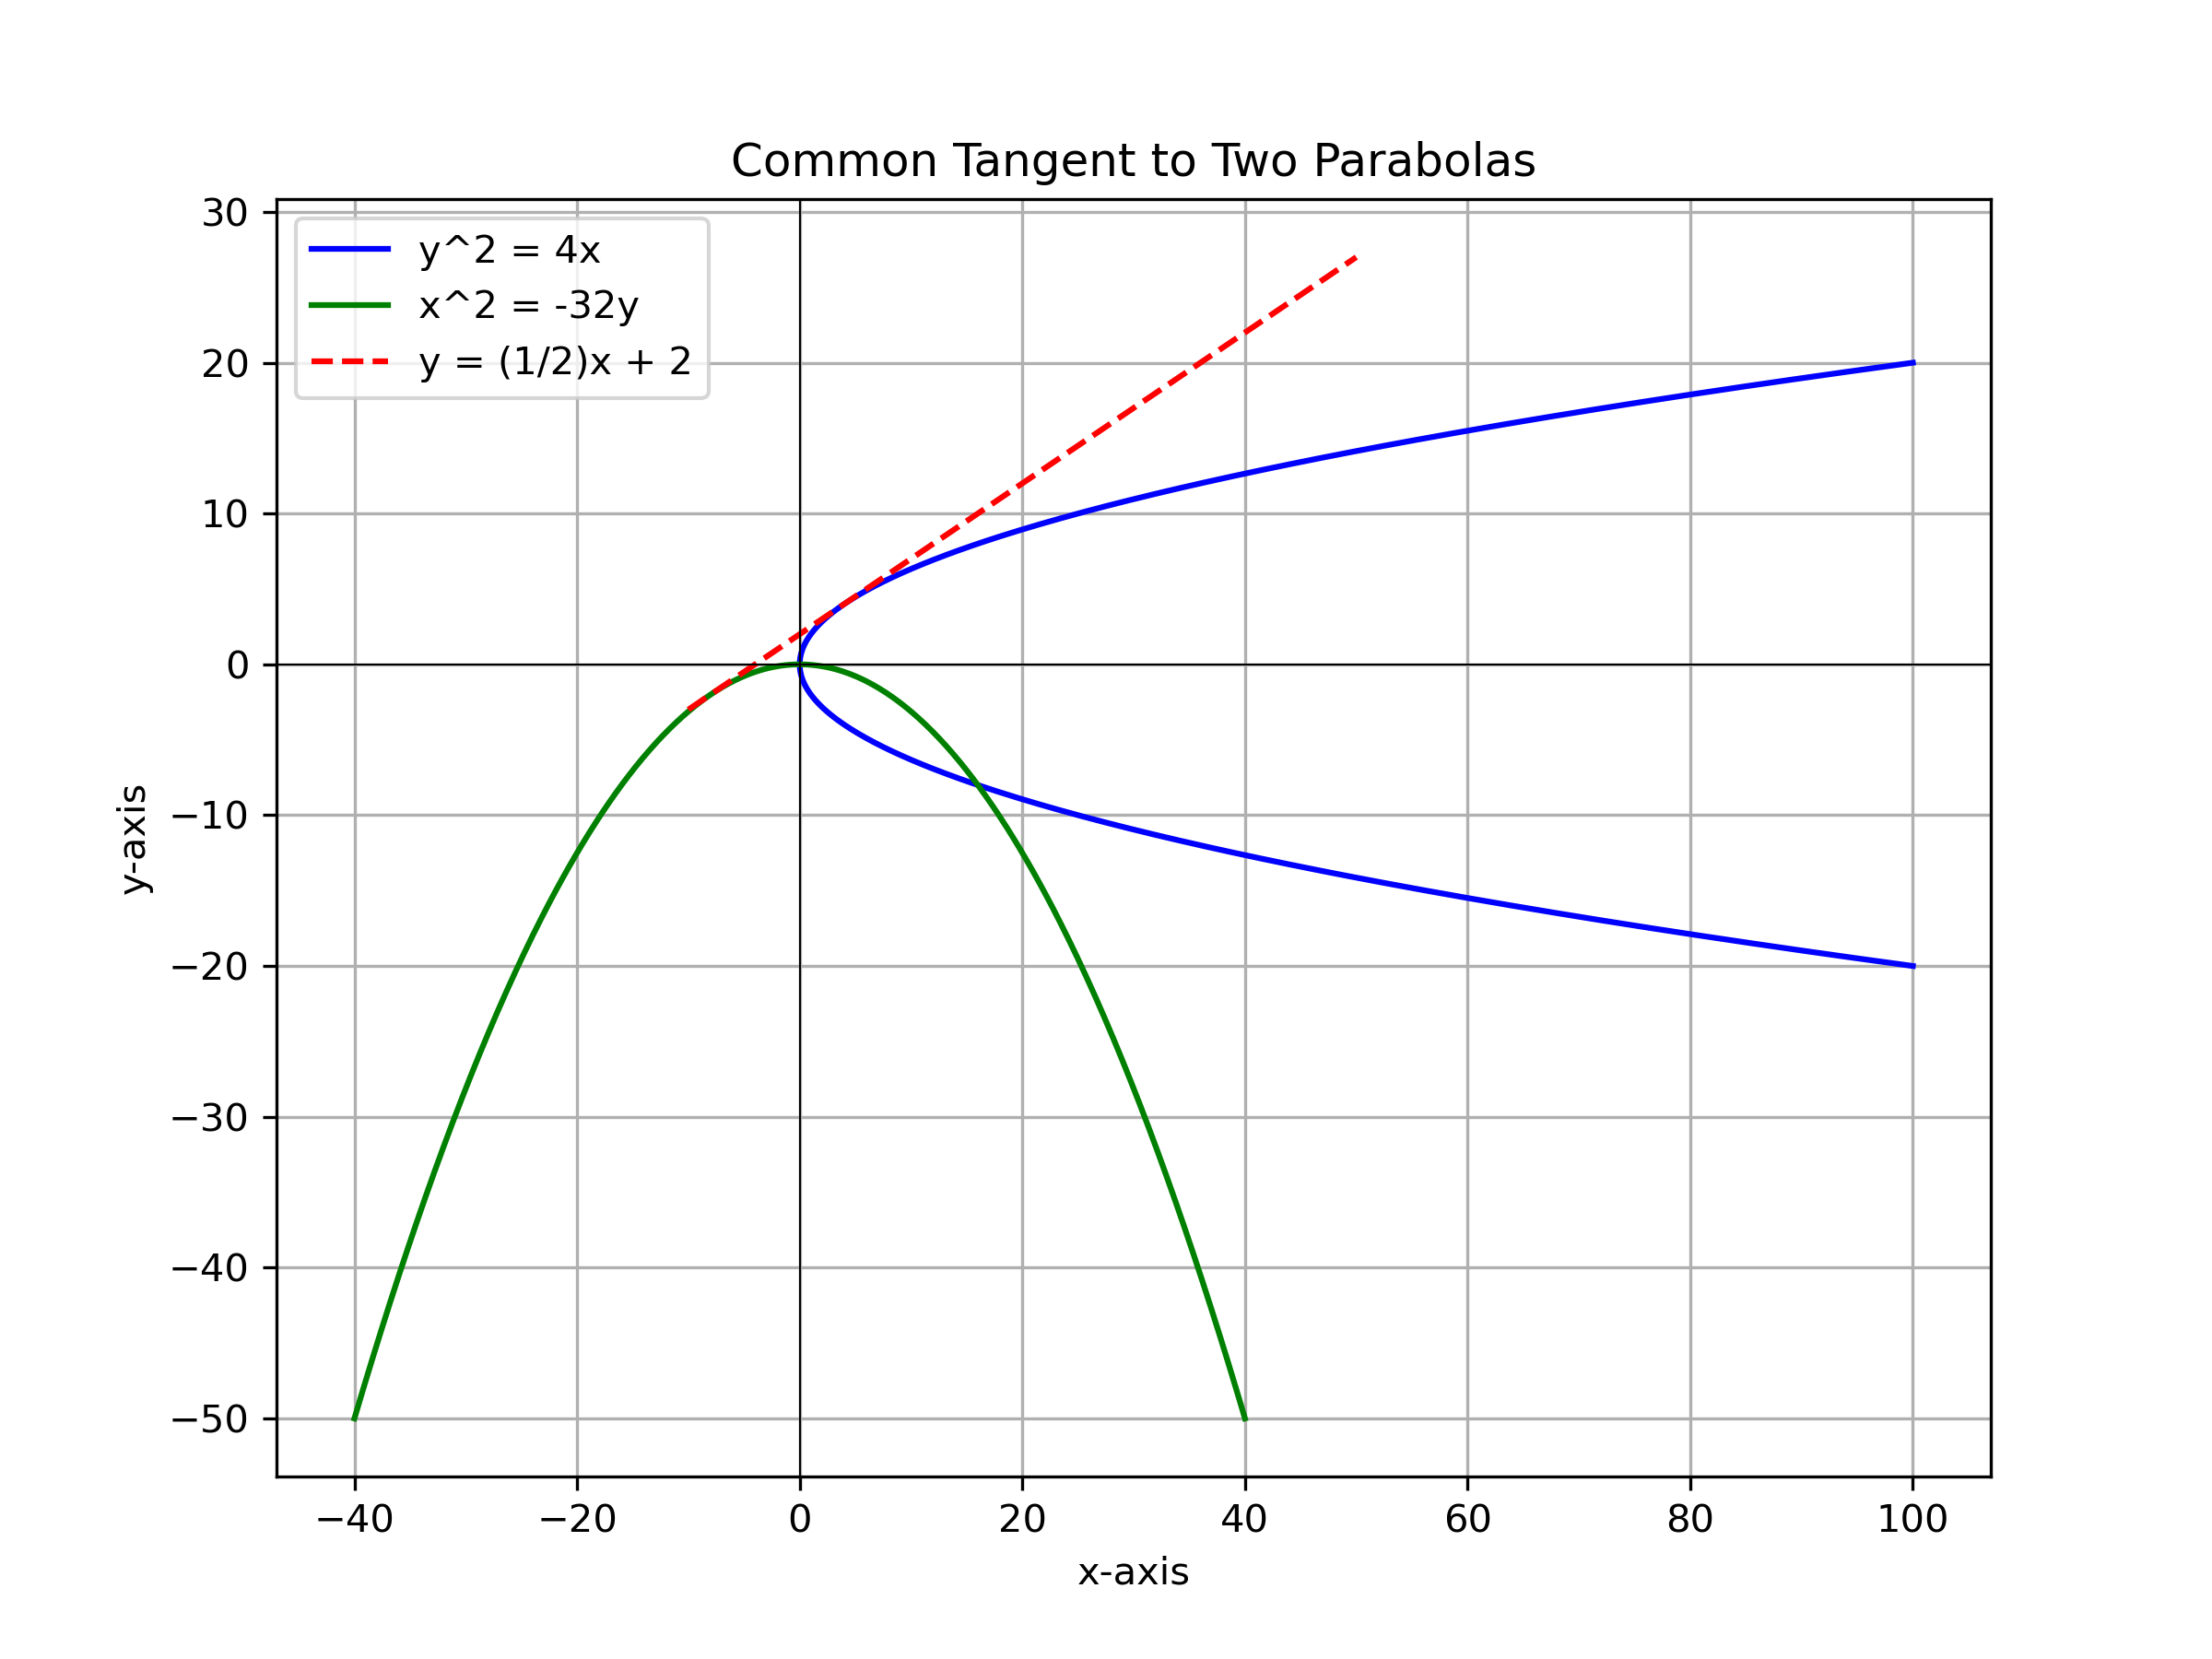
\includegraphics[width=0.9\columnwidth]{figs/01.png}
    \caption{}
    \label{fig:placeholder}
\end{figure}
\end{frame}
% --------- CODE APPENDIX ---------
\section*{Appendix: Code}

% C program
\begin{frame}[fragile]{C Code: Slope.c}
\begin{lstlisting}[language=C]
#include <stdio.h>
#include <math.h>

int main() {
    FILE *fp;
    double m;

    // Calculation based on derived formula: m^3 = 1/8
    m = cbrt(1.0/8.0);  // cube root

    // Open file slope.dat for writing
    fp = fopen("slope.dat", "w");
    if(fp == NULL) {
        printf("Error opening file!\n");
        return 1;
    }

    // Write slope value into file
    fprintf(fp, "The slope of the common tangent is: %lf\n", m);

    fclose(fp);

    printf("Result written to slope.dat successfully.\n");
    return 0;
}


    \end{lstlisting}
\end{frame}

% Python plotting
\begin{frame}[fragile]{Python: plot.py}
\begin{lstlisting}[language=Python]
import numpy as np
import matplotlib.pyplot as plt

# Define parabola 1: y^2 = 4x  -> x = y^2 / 4
y1 = np.linspace(-20, 20, 400)
x1 = (y1**2) / 4

# Define parabola 2: x^2 = -32y -> y = -x^2 / 32
x2 = np.linspace(-40, 40, 400)
y2 = -(x2**2) / 32

# Define common tangent: y = (1/2)x + 2
x_tan = np.linspace(-10, 50, 400)
y_tan = 0.5 * x_tan + 2

# Plot the parabolas
plt.figure(figsize=(8, 6))
plt.plot(x1, y1, 'b', label='y^2 = 4x')
plt.plot(x2, y2, 'g', label='x^2 = -32y')

# Plot the tangent line
plt.plot(x_tan, y_tan, 'r--', label='y = (1/2)x + 2')
plt.xlabel("x-axis")
plt.ylabel("y-axis")
plt.title("Common Tangent to Two Parabolas")
plt.axhline(0, color='black', linewidth=0.5)
plt.axvline(0, color='black', linewidth=0.5)
plt.legend()
plt.grid(True)
plt.savefig("slope_plot.png", dpi=300)
# Show the plot
plt.show()

\end{lstlisting}
\end{frame}

\end{document}
